\chapter{Game Theory}
\label{chap:game-theory}

\begin{lemma}
	For every game $G$, there exists at least one individually rational strategy profile.
	In other words, $\mathcal{S}_1(G) \ne \emptyset$.
\end{lemma}

\begin{proof}
	For every player $i \in P$ we denote $m_i \in S_i$ the strategy that lower-bounds utility of player $i$:
	\[
		m_i = \text{arg} \max_{t_i \in S_i} \min_{\vect_{-i} \in S_{-i}} u_i(t_i, \vect_{-i}).
	\]
	We claim that the strategy profile $\mm = (m_1, \dots, m_n) \in S$ is individually rational.
	If $\mm$ was not individually rational, there would have to be some player $j \in P$ and a strategy $s_j^* \in S_j$ that would ensure a better worst-case payoff: $\min_{\vecs_{-j} \in S_{-j}}u_j(s_j^*, \vecs_{-j}) > u_j(\mm)$ which would contradict the choice of~$m_j$.
\end{proof}

In this chapter, we introduce two new equilibria: the perfectly transparent best response equilibrium, and the perfectly transparent best profile equilibrium.
Then, we discuss some relations between these two equilibiria, and between the other equilibria introduced in \autoref{chap:background}.

\begin{definition}[Perfectly transparent best response]
	In a game $G = (P, S, \uu)$ we say a strategy $s_i^* \in S_i$ is a perfectly transparent best response to a strategy profile $\vecs_{-i} \in S_{-i}$ of the opponent players if it is the Nashian best response to $\vecs_{-i}$ across all profiles that survive the maximum number of preemption rounds.
	The weak/strict notion is inherited from the Nashian best response.
	Formally $s_i^*$ is a (\textit{weak}) perfectly transparent best response if either $(s_i^*, \vecs_{-i})$ is a PTE or $\exists k \in \N: (s_i^*, \vecs_{-i}) \in \mathcal{S}_k(G), (s_i, \vecs_{-i}) \notin \mathcal{S}_{k+1}(G) \forall s_i \in S_i$, and
	\[
		\forall (s_i', \vecs_{-i}) \in \mathcal{S}_k(G): u_i(s_i^*, \vecs_{-i}) \ge u_i(s_i', \vecs_{-i}).
	\]
	It is a \textit{strict} perfectly transparent best response if either $(s_i^*, \vecs_{-i})$ is a PTE or $\exists k \in \N: (s_i^*, \vecs_{-i}) \in \mathcal{S}_k(G), (s_i, \vecs_{-i}) \notin \mathcal{S}_{k+1}(G) \forall s_i \in S_i$, and
	\[
		\forall (s_i', \vecs_{-i}) \in \mathcal{S}_k(G): s_i' \ne s_i^* \implies u_i(s_i^*, \vecs_{-i}) > u_i(s_i', \vecs_{-i}).
	\]
\end{definition}

\begin{definition}[Perfectly transparent best response equilibrium]
	We say a strategy profile $\vecs = (s_1, \dots, s_n) \in S$ is a (\textit{weak}) perfectly transparent best response equilibrium (PTBRE) if $s_i$ is a (weak) perfectly transparent best response to $\vecs_{-i}$ for all players $i \in P$.
	
	Similarly, $\vecs$ is a \textit{strict} PTBRE if $s_i$ is a strict perfectly transparent best response to $\vecs_{-i}$ for all players $i \in P$.
\end{definition}

\begin{definition}[Perfectly transparent $i$-best profile]
	For a givne game $G = (P, S, \uu)$ and player $i \in P$ we say a strategy profile $\vecs = (s_1, \dots, s_n) \in S$ is a (\textit{weak}) perfectly transparent $i$-best profile if
	$s_i$ is a (weak) perfectly transparent best response to $\vecs_{-i}$ and
	\[
		\forall \vecs'_{-i} \in S_{-i}: u_i(\vecs) \ge u_i\left(b(\vecs'_{-i}), \vecs'_{-i}\right),
	\]
	where $b(\vecs'_{-i})$ is the perfectly transparent best response to $\vecs'_{-i}$.
	It is a \textit{strict} perfectly transparent $i$-best profile if $s_i$ is a strict perfectly transparent best response to $s_{-i}$ and
	\[
		\forall \vecs_{-i}' \in S_{-i}: \vecs_{-i}' \ne s_{-i} \implies u_i(\vecs) > u_i\left(b(s_{-i}'), \vecs_{-i}'\right).
	\]
\end{definition}

\begin{definition}[Perfectly transparent best profile equilibrium]
	We say that a strategy profile $\vecs \in S$ is a (\textit{weak}) perfectly transparent best profile equilibrium (PTBPE) if $\vecs$ is a (weak) perfectly transparent $i$-best profile for all $i \in P$.

	Similarly, $\vecs$ is a \textit{strict} PTBPE if it is a strict perfectly transparent $i$-best profile for all $i \in P$.
\end{definition}

Recall that for any game $G = (P, S, \uu)$, a strategy profile $\vecs \in S$ is individually rational if and only if it survives the first preemption round: $\vecs \in \mathcal{S}_1(G)$.
This means that every PTE must be individually rational.
If we think of these equilibiria as sets of strategy profiles in any possible game, we can express this as PTE $\subset$ IR.
It is not hard to see that the inclusion is indeed strict as there are games in which $\mathcal{S}_2 \subsetneq \mathcal{S}_1$, so not all individually rational profiles are PTEs.

In the rest of this chapter, we present several such inclusion results that help to understand the relations between individal rationality, perfetcly transparent best response equilibiria, perfectly transparent equilibiria, perfectly transparent best profile equilibiria, and minimax rationalizibility.

\section{Games without ties}
We can observe that in games without ties, similar to Nash equilibria, weak and strict equilibiria are equivalent also in the case of PTBRE and PTBPE.
Thus, in this section, we do not distingiush between them.

\begin{lemma}
	For any game $G = (P, S, \uu)$, if a strategy profile $\vecs \in S$ is a PTBRE, then it is individually rational.
	Thus, we have PTBRE $\subset$ IR.
\end{lemma}

\begin{proof}
	Let us suppose that there is a game $G = (P, S, \uu)$ and a strategy profile $\vecs = (s_1, \dots, s_n) \in S$ such that $\vecs$ is a PTBRE but not individually rational.
	This is equivalent to $s_i$ being a perfectly transparent best response to $\vecs_{-i}$ for all $i \in P$, and $\vecs \notin \mathcal{S}_1(G)$.
	Note that we must also have $(s_i', \vecs_{-i}) \notin \mathcal{S}_1(G)\ \forall s_i' \in S_i,\ \forall i \in P$ because otherwise $s_i$ would not be a perfectly transparent best response to $\vecs_{-i}$ for some player $i$.
	This means the perfetcly transparent best response of every player $i \in P$ to $\vecs_{-i}$ is simply a Nashian best response (since all considered strategy profiles are eliminated in the same preemption round).
	Thus, $\vecs$ is a Nash equilibrium, which is always individually rational.
\end{proof}

\begin{remark}
	\autoref{tab:ir-ne-ptbre} shows that the inclusion is indeed strict.
\end{remark}

\begin{observation}
	\label{th:ptbre-subset-pte}
	If a strategy profile is a PTE, then it must be a PTBRE; we have PTE $\subset$ PTBRE.
\end{observation}

\begin{remark}
	\autoref{tab:ptbre-ne-pte} shows that the inclusion is strict.
\end{remark}

\begin{lemma}
	If a game $G = (P, S, \uu)$ has a PTBPE $\vecs \in S$, then $\vecs$ is also a PTE, i.e., we have the inclusion PTBPE $\subset$ PTE.
\end{lemma}

\begin{proof}
	For the sake of deriving a contradiction, suppose that there is a game $G = (P, S, \uu)$ with a strategy profile $\vecs = (s_1, \dots, s_n) \in S$ such that $\vecs$ is a PTBPE but not a PTE and let $k$ be the last preemption round in which $\vecs$ is not eliminated (i.e., $\vecs \in \mathcal{S}_k(G)$ but $\vecs \notin \mathcal{S}_{k+1}(G)$).
	Because $\vecs$ is eliminated in the $(k+1)$\textsuperscript{st} round, there must be some player $i \in P$ with a strategy $s_i^* \ne s_i$ which causes the elimination:
	\[
		\forall \vecs_{-i}' \in S_{-i}: (s_i^*, \vecs_{-i}') \in \mathcal{S}_k(G) \implies u_i(s_i^*, \vecs_{-i}') > u_i(\vecs).
	\]
	Let $\vecs_{-i}^* \in S_{-i}$ such that $(s_i^*, \vecs_{-i}^*)\in \mathcal{S}_k(G)$ (there must be at least one to cause $\vecs \notin \mathcal{S}_{k+1}(G)$).
	We have $u_i(s_i^*, \vecs_{-i}^*) > u_i(\vecs)$ which means $s_i$ is not a perfectly transparent best response of player $i$ to $\vecs_{-i}$, so $\vecs$ is not a perfectly transparent $i$-best profile, contradicting $\vecs$ being a PTBPE.
\end{proof}

\begin{remark}
	\autoref{tab:pte-ne-ptbpe} shows that the inclusion is strict.
\end{remark}

Minimax rationalizibility intersects with all the other equilibiria, as shown in \autoref{tab:ptbpe-ne-minimax} and \autoref{tab:ptbpe-eq-minimax}.

\begin{figure}
	\caption{A venn diagram depicting the inclusion of different equilibria.}
	\centering

	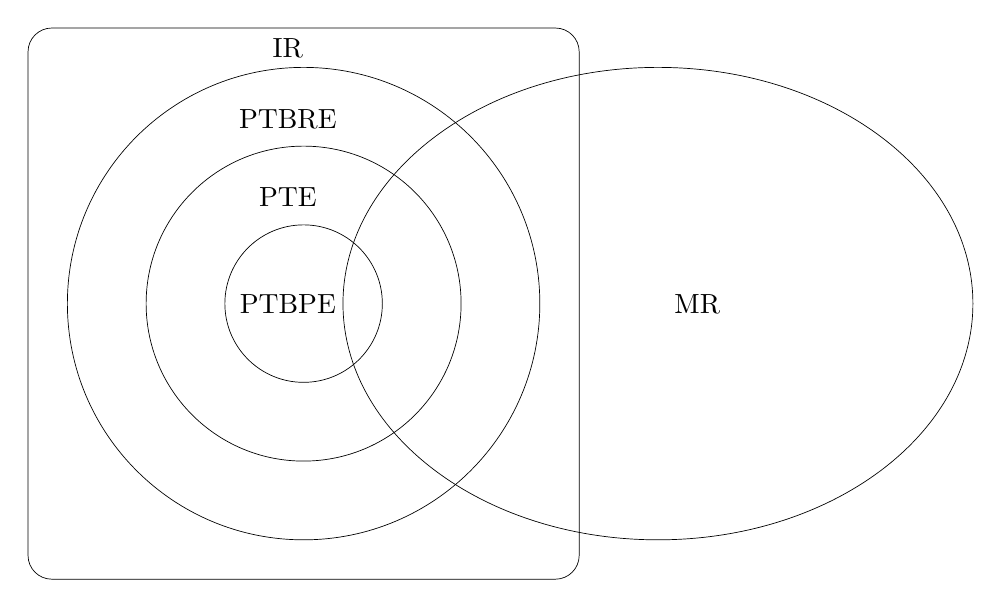
\begin{tikzpicture}[line width=0.25pt]
		\draw (0,0) circle (1);
		\draw (0,0) circle (2);
		\draw (0,0) circle (3);
		\draw[rounded corners=2ex] (-3.5,3.5) rectangle (3.5,-3.5);
		\draw (4.5,0) ellipse (4 and 3);
		\node at (-0.2,0) {PTBPE};
		\node at (-0.2,1.35) {PTE};
		\node at (-0.2,2.35) {PTBRE};
		\node at (-0.2,3.25) {IR};
		\node at (5,0) {MR};
	\end{tikzpicture}
\end{figure}

\section{Symmetric games without ties}

\begin{observation}
	 In a symmetric game $G = (P, S, \uu)$, if a strategy profile $\vecs \in S$ is a PTE, then it lies on the diagonal, i.e., we have $\vecs = (a, a, \dots, a)$ for some strategy $a$.
\end{observation}

\begin{proof}
	If there was a PTE somewhere else than on the diagonal, we would necessarily have multiple PTEs by symmetry, contradicting the uniqueness of PTE.
\end{proof}

\begin{corollary}
	If a symmetric game $G = (P, S, \uu)$ has a PTE $\vecs \in S$ and $\vecs$ is the perfectly transparent $i$-best profile for some player $i \in P$, then $\vecs$ is a PTBPE. 
\end{corollary}

\begin{proof}
	Since $\vecs$ is on the diagonal and it is the perfectly transparent $i$-best profile for some $i \in P$, by symmetry, it must actually be the perfectly transparent $j$-best profile for all $j \in P$, which is the definition of PTBPE.
\end{proof}

\begin{lemma}
	In a symmetric game $G = (P, S, \uu)$, if a strategy profile $\vecs \in S$ is a PTE, then it is minimax rationalizable.
	Thus, we have PTE\textsuperscript{sym} $\subset$ MR.
\end{lemma}

\begin{proof}
	Suppose for the sake of deriving a contradiction that there is a game $G = (P, S, \uu)$ and a strategy profile $\vecs \in S$ that is a PTE but not minimax rationalizable.
	By definition, this means that there is some player $i \in P$ such that $(s_i, \vecs_{-i}')$ is not minimax rationalizable for any $\vecs' \in S$.
	By symmetry, if this statement holds for one player, then it must hold for all players.
	Let $s_j$ be the strategy that minimax-dominates $s_i$ (i.e. causes that $s_i$ is not minimax rationalizable).
	We denote $\vecs^* = (s_j, s_j, \dots, s_j)$.
	In the round where strategy $s_i$ is eliminated, strategy profile $\vecs^*$ must survive---otherwise strategy $s_j$ would be eliminated as well, but we supposed that $s_j$ is the strategy that caused the elimination of $s_i$.
	Moreover, we must have $u_i(\vecs^*) > u_i(\vecs)\ \forall i \in P$ because $s_j$ minimax-dominates $s_i$.
	This means $\vecs$ is not Pareto-optimal which contradicts $\vecs$ being a PTE.
\end{proof}
